\section{Analysis of a Genuine Planned-Missing Archive}\label{app:pisa}
\begin{table}[t]
\centering
\caption{PISA secondary analysis on 2,441 held-out students. Brier improvement and 95\% intervals are multiplied by $10^3$; positive means the newer rule has smaller loss. Survey intervals use the 80 supplied Fay replicates. MI intervals also use Rubin combination under a working imputation model.}
\label{tab:pisa}
\small
\begin{tabular}{lrr}
\toprule
Method & Estimate & 95\% interval \\
\midrule
Form score & 1.13 & $[-2.28, 4.53]$ \\
Block/pair HT & 1.24 & $[-2.09, 4.57]$ \\
Logistic MI & 1.24 & $[-2.12, 4.60]$ \\
\bottomrule
\end{tabular}
\end{table}

\subsection{Observed forms, common target and acquisition constraint}
We use the national U.S. PISA 2012 student public-use file supplied by NCES
\citep{pisaus2014}. The OECD technical report, Chapter 3, describes random
allocation of three student questionnaires, with approximately equal
counts. Each has an eight-minute common part and two eleven-minute rotated
parts. The U.S. technical report describes the forms' A--B--C spiraling
and the required survey-weight analysis \citep{pisa2014,kastberg2014}.
Our analysis uses allocation probabilities $q_A=q_B=q_C=1/3$. The observed
form identifier is \texttt{QUESTID}; \texttt{FORMID} identifies a different,
computer-based assessment and must not be used for this purpose.

The nine predictors are the first three response items in each of
\texttt{ST29} (interest/motivation), \texttt{ST42} (anxiety/self-concept),
and \texttt{ST53} (learning strategies). Call these blocks $U,V,W$.
Forms A, B, C reveal $(U,W)$, $(U,V)$, $(V,W)$, respectively. The released
codes confirm that every selected item outside its assigned form has the
structural not-applicable code. Within a received form, ST29/ST42 responses
1 or 2 define endorsement; ST53 response 1 defines endorsement. All other
received responses, including item nonresponse or invalid codes, define
nonendorsement. Thus we estimate a contrast of recorded responses, not
the unobserved substantive answers of nonresponders. This convention does
not complete any structurally omitted block.

The common target \texttt{ST07Q01} asks about grade repetition in grades
1--6. Codes 2/3 define $Z=1$, and code 1 defines $Z=0$. We retain 4,752 of
4,978 records with a valid target report. The design-based interpretation
is conditional on this respondent population and assumes that common-part
response does not break the randomized allocation. A claim about all
students, including target nonresponders, would require further assumptions.
There are 1,582/1,590/1,580 retained records on A/B/C. No record has all
nine selected predictors. These are nine selected indicators within a
larger 30-minute questionnaire, not nine independent tests in the actual
survey protocol.

\subsection{Frozen ensembles trained from incomplete records}
We permute the 162 school IDs with seed 20261108. The first forty schools
train the old rule, the next forty train the new rule, and the remaining
82 form the audit domain. The corresponding valid-target record counts
are 1,115, 1,196 and 2,441. The audit contains 801/821/819 A/B/C forms.
School-level separation avoids training and evaluating on students in
the same school. Estimates and uncertainty below condition on the fitted
rules and the chosen audit domain; they do not include variation from
retraining the models.

For version $j\in\{0,1\}$, let
\[
 p_j(x)=\{f_{jU}(x_U)+f_{jV}(x_V)+f_{jW}(x_W)\}/3.
\]
Each component is a fifty-tree probability forest, trained only on records
receiving that block. Old/new component depths are two/three, respectively,
with minimum leaf size twenty, all three block features eligible at each
split, fixed independent seeds, and survey weights normalized to mean
one in fitting. Old block fits use 745/744/741 records; new fits use
805/786/801. There is no complete-record training or calibration sample.
The resulting contrast depends on all nine predictors. This is a
specified secondary model-comparison task, not a deployed educational
prediction system or a causal analysis of grade repetition.

\subsection{Why Brier comparison is identifiable on these actual forms}
For $K=3$ blocks, set
\[
 a_k=\frac{f_{0k}^2-f_{1k}^2}{9}
       +\frac{2Z}{3}(f_{1k}-f_{0k}),\qquad
 b_{k\ell}=\frac{2}{9}(f_{0k}f_{0\ell}-f_{1k}f_{1\ell}).
\]
Expanding the squared losses gives the pointwise identity
\[
 (p_0-Z)^2-(p_1-Z)^2=\sum_k a_k+\sum_{k<\ell}b_{k\ell}.
\]
Every single block is observed with probability $2/3$ and every pair with
probability $1/3$. On the form containing $k,\ell$, the score
$\tfrac32(a_k+a_\ell)+3b_{k\ell}$ is consequently unbiased. For randomized
accuracy the corresponding score is
$\tfrac{Y}{2}\{(f_{1k}-f_{0k})+(f_{1\ell}-f_{0\ell})\}$.
Both are evaluated entirely on received responses and the common label.

The same argument applies to an average of arbitrary block functions:
accuracy requires coverage of each block; Brier additionally requires
coverage of each interacting block pair. This is an application of the
observation-span criterion. A nonlinear transformation such as log loss
can involve three-block interactions that none of these forms observes.
The fact that every pair of blocks co-occurs does not identify arbitrary
functions of all three blocks.

For the optimized score, keep $q=1/3$ and solve the quadratic version of
\eqref{eq:fullprogram}. Each form has 64 binary cells; 169 distinct Fourier
terms occur across the three forms. The constraints are imposed separately
for the two labels. Estimate each form's joint cell--label frequencies
from the pooled old/new training schools, using survey weights within
that form and 0.1 uniform shrinkage. No assumption that these estimated
marginals form a compatible joint distribution is needed for unbiasedness.
The released tables satisfy the target identity on all 512 profiles and
both labels; the maximum numerical residual is $3.1\times10^{-16}$.

\subsection{Survey uncertainty and imputation comparator}
Let $w_i$ and $w_i^{(r)}$ be the supplied final and eighty replicate
weights. For frozen scores $H_i$, report the weighted mean
$\widehat\Delta=\sum_iw_iH_i/\sum_iw_i$ in the audit domain and
\[
 \widehat{\operatorname{se}}^2
 =\frac{1}{80(1-0.5)^2}
       \sum_{r=1}^{80}(\widehat\Delta^{(r)}-\widehat\Delta)^2.
\]
This is the documented Fay BRR calculation, not an iid Wald calculation.
The resulting normal intervals are survey-asymptotic intervals, not the
finite-sample minimax confidence guarantee. Conditional on sampled records
and their fixed weights, the weighted form-score mean is unbiased over
the stipulated form assignment; survey-population interpretation also
uses the survey's weighting and response assumptions.

We implement twenty independent chains of logistic multiple imputation
\citep{vanbuuren2011}, with fifteen sweeps per chain and fixed seeds. Only
the omitted block is imputed. Each conditional regression uses the other
eight predictors, observed target, reported sex, grade and log survey
weight. Coefficients use Laplace draws around a weakly regularized,
weighted logistic fit. This is a transparent working-model implementation,
not a claim to run the R \texttt{mice} package or an exact posterior sampler.
For each completed dataset we evaluate the frozen contrast and its Fay
variance. Rubin combination uses within-imputation mean variance
$\overline U$, between-imputation variance $B$, total
$\overline U+(1+1/20)B$, and the usual degrees-of-freedom adjustment.
These intervals depend on the imputation specification, its compatibility
with the target, and survey approximations; nominal coverage is not
verified without complete-data truth.

For randomized accuracy, optimized scores give 0.04142 with interval
$[0.03785,0.04500]$, block HT gives 0.04174 with
$[0.03814,0.04534]$, and logistic MI gives 0.04180 with
$[0.03825,0.04535]$. For Brier improvement, all intervals in
Table~\ref{tab:pisa} contain zero. Both probabilities stay below 0.5 on
the full cube (old range 0.112--0.231, new range 0.040--0.137), so
thresholded accuracy has identically zero contrast. The probability-loss
comparison is substantive only as a probability-quality target, not as
an improvement in these deterministic decisions. The agreement is useful evidence of
stability for this specified analysis, not evidence that the imputation
model is correct or that optimized scores dominate simpler scores.

Each predictor occurs on two forms, allowing nine marginal response
comparisons. On audit records, two unadjusted BRR comparisons have
$p<0.05$ (0.0479 and 0.0449); none meets $0.05/9$. The maximum estimated
difference is 0.0482. Random differences, form order, context and
nonresponse can all contribute. Failure to reject after correction does
not certify measurement invariance, and these marginal checks cannot
identify all unobserved joint response differences. No branching benefit,
MSE or coverage estimate is claimed from this archive.

\section{Cost Regimes Under a Relaxable Cap}\label{app:costchoice}
\begin{figure}[ht]
\centering
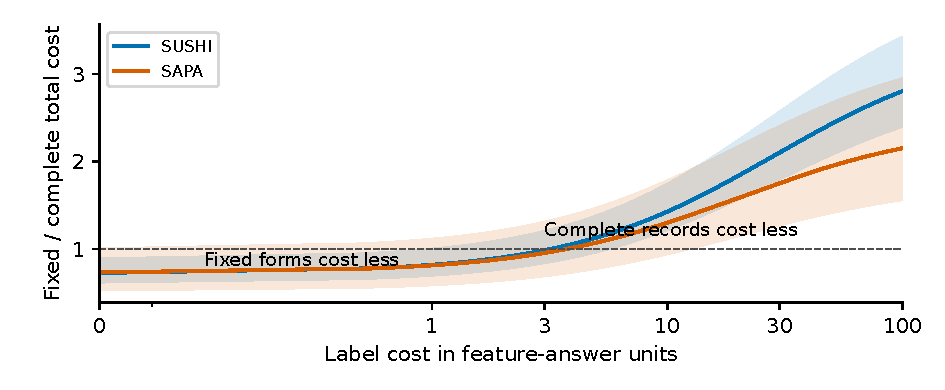
\includegraphics[width=.85\textwidth]{figures/cost_choice.pdf}
\caption{Fixed-form versus complete-record cost on all 70 controlled tree
tasks, allowing complete acquisition. Lines are medians, bands are the
10th--90th percentiles. Planning targets half-width 0.025, includes integer
sample counts and a minimum of thirty, and conditions on the reference.
Under an immutable cap, the complete-record alternative is unavailable.
When branching can compute the target and is permitted, its lower feature
count and full-information variance make it the natural comparator.}
\label{fig:costchoice}
\end{figure}
At zero label cost the median planned fixed/complete ratios are 0.726 on
SUSHI and 0.731 on SAPA; at label cost ten they are 1.427 and 1.299.
These conditional cost curves do not price an independent complete
reference as free: same-population reference records should first be used
as audit observations. Transferred or restricted calibration requires its
own analysis. An uncorrected imputation method cannot be assigned a
universal winning region using label cost alone, because its bias,
sample size and desired inference guarantee also matter.
